\begin{frame}{Surface X-ray diffraction}
    \begin{columns}
        \column[T]{0.35\textwidth}
        \centering
        \begin{itemize}
            \item SXRD allows us to probe the last layers of the crystal structure
            \vspace{0.5cm}
            \pause
            \item Study \textcolor{Important}{single facets} with the same setup and conditions, Pt (100), (111), ...
            % \pause
            % \item Expected results are surface reconstructions and the formation of new surface structures
            \vspace{0.5cm}
            \pause
            \item \textcolor{Important}{Explore correlation between specific facets and reaction products}
        \end{itemize}

        \centering
        \pause
        \begin{figure}
            \centering
            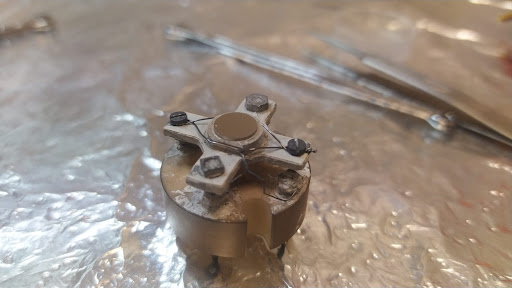
\includegraphics[width=0.9\textwidth, trim={3.5cm 3.5cm 5cm 3.5cm}, clip]{Figures/sxrd_data/sample_sxrd.jpg}
            \caption{Pt monocrystal used during Surface X-ray Diffraction.}
            \label{fig:my_label}
        \end{figure}

        % \pause
        % \begin{figure}
        %     \centering
        %     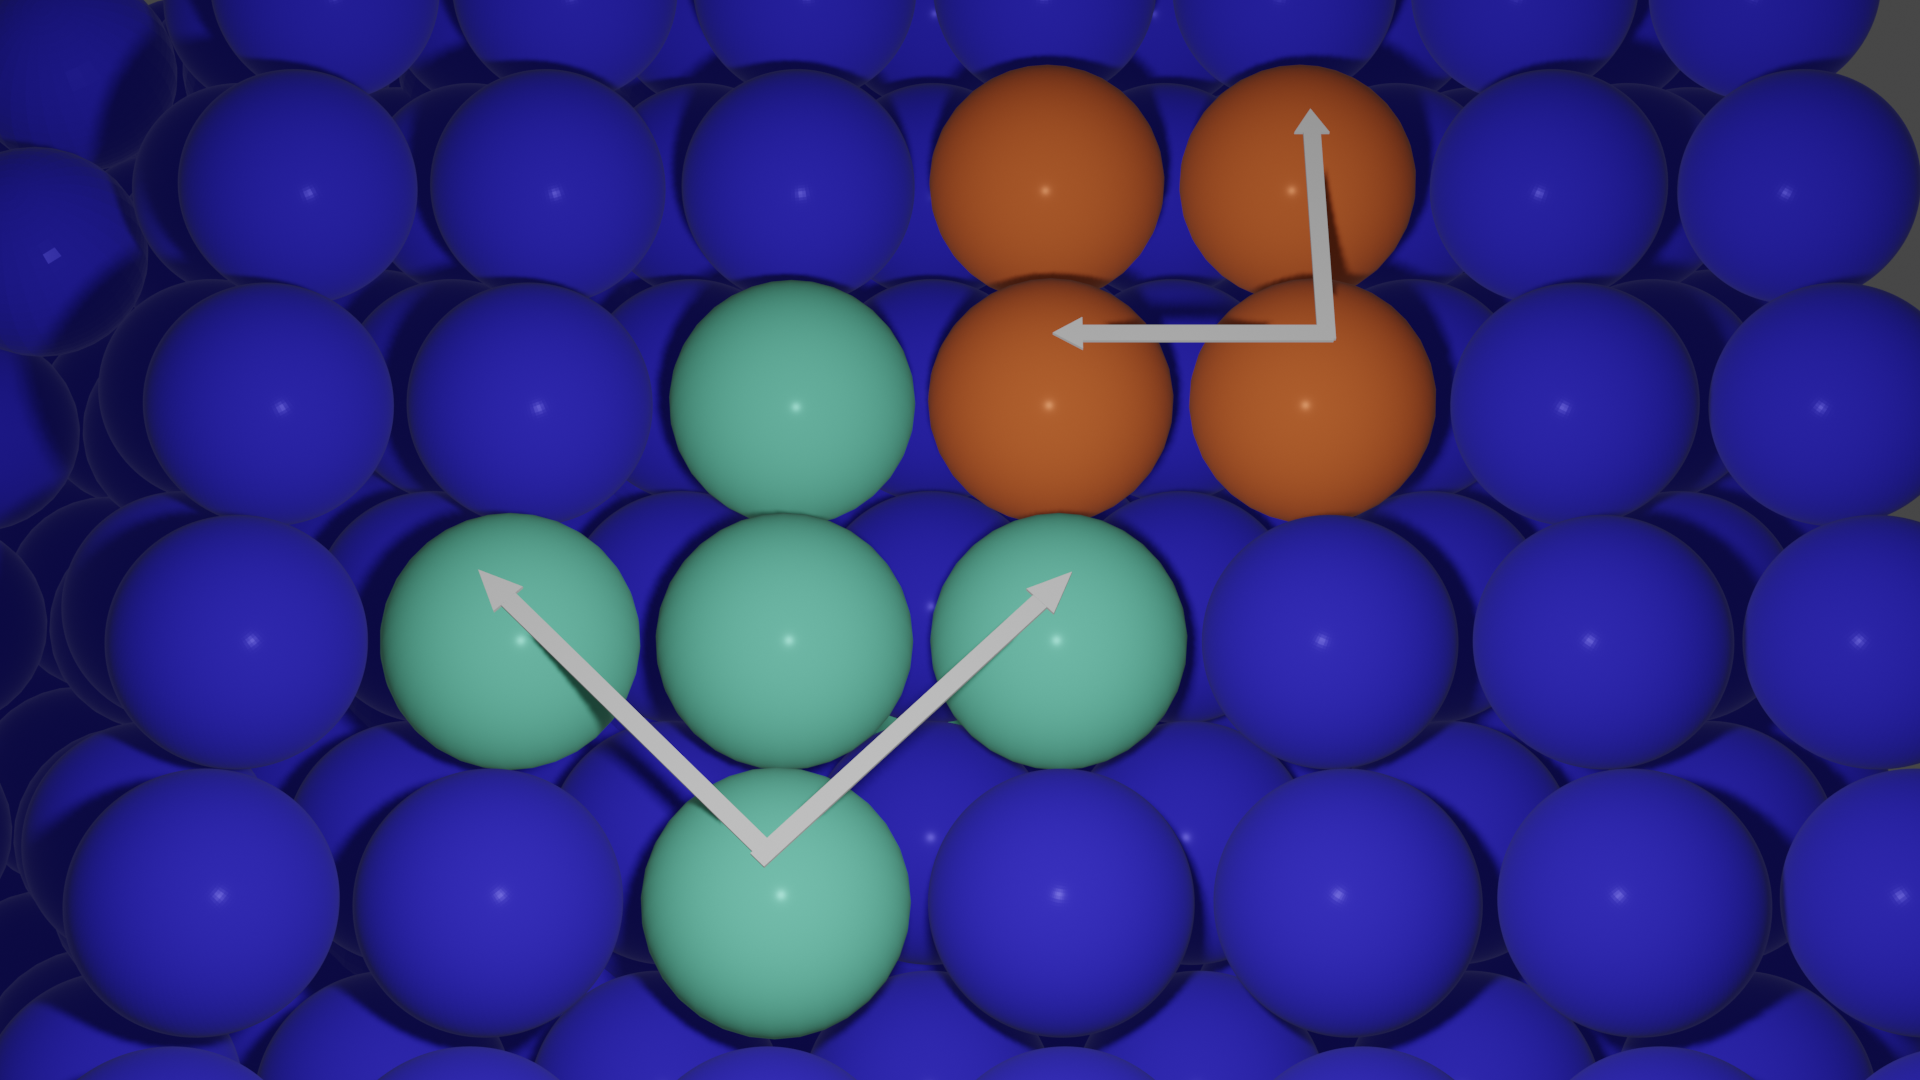
\includegraphics[width=0.8\textwidth]{Figures/sxrd_data/Pt100_blender.png}
        %     \caption{Pt (001) bulk unit cell (green) and surface unit cell (orange).}
        %     \label{fig:pt100_unit_cells}
        % \end{figure}

        \column[T]{0.65\textwidth}
        \pause
        \begin{figure}
            \centering
            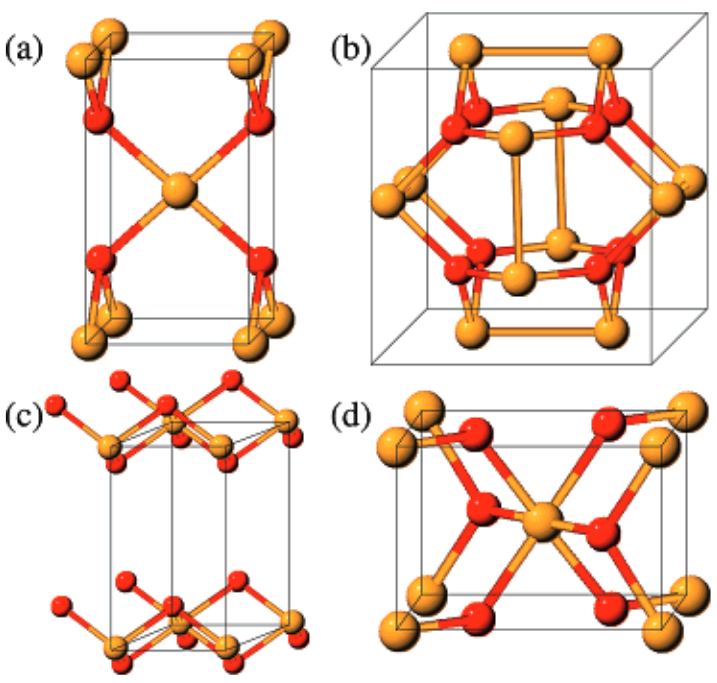
\includegraphics[width=0.65\textwidth]{Figures/sxrd_data/PtOxides.png}
            \caption{Crystal  structure  of  platinum  oxides expected on Pt (100): (a) $PtO$; (b) \ptthreeofour;(c) $\alpha-PtO_2$; and (d) $\beta-PtO_2$ \footnotemark{}.\\ \textcolor{orange}{Platinum} and \textcolor{red}{Oxygen} atoms.}
            \label{fig:PtOstructures}
        \end{figure}

        \footnotetext{$^3$ Seriani, N., Pompe, W., Ciacchi, L. (2006). Catalytic oxidation activity of Pt3O4 surfaces and thin films. Journal of Physical Chemistry B, 11(30), 14860–14869.}

    \end{columns}
    
\end{frame}